\documentclass{article}

\def\npart{II}
\def\nyear{2017}
\def\nterm{Michaelmas}
\def\nlecturer{Prof. P. Russell}
\def\ncourse{Graph Theory}
\ifx \nauthor\undefined
  \def\nauthor{Bhavik Mehta}
\else
\fi

\author{Based on lectures by \nlecturer \\\small Notes taken by \nauthor}
\date{\nterm\ \nyear}
\title{Part \npart\ -- \ncourse}

\usepackage[utf8]{inputenc}
\usepackage{amsmath}
\usepackage{amsthm}
\usepackage{amssymb}
\usepackage{enumerate}
\usepackage{mathtools}
\usepackage{graphicx}
\usepackage[dvipsnames]{xcolor}
\usepackage{tikz}
\usepackage{wrapfig}
\usepackage{centernot}
\usepackage{float}
\usepackage{braket}
\usepackage[hypcap=true]{caption}
\usepackage{enumitem}
\usepackage[colorlinks=true, linkcolor=mblue]{hyperref}
\usepackage[nameinlink,noabbrev]{cleveref}
\usepackage{nameref}
\usepackage[margin=1.5in]{geometry}

% Theorems
\theoremstyle{definition}
\newtheorem*{aim}{Aim}
\newtheorem*{axiom}{Axiom}
\newtheorem*{claim}{Claim}
\newtheorem*{cor}{Corollary}
\newtheorem*{conjecture}{Conjecture}
\newtheorem*{defi}{Definition}
\newtheorem*{eg}{Example}
\newtheorem*{ex}{Exercise}
\newtheorem*{fact}{Fact}
\newtheorem*{law}{Law}
\newtheorem*{lemma}{Lemma}
\newtheorem*{notation}{Notation}
\newtheorem*{prop}{Proposition}
\newtheorem*{question}{Question}
\newtheorem*{rrule}{Rule}
\newtheorem*{thm}{Theorem}
\newtheorem*{assumption}{Assumption}

\newtheorem*{remark}{Remark}
\newtheorem*{warning}{Warning}
\newtheorem*{exercise}{Exercise}

% \newcommand{\nthmautorefname}{Theorem}

\newtheorem{nthm}{Theorem}[section]
\newtheorem{nlemma}[nthm]{Lemma}
\newtheorem{nprop}[nthm]{Proposition}
\newtheorem{ncor}[nthm]{Corollary}
\newtheorem{ndef}[nthm]{Definition}

% Special sets
\newcommand{\C}{\mathbb{C}}
\newcommand{\N}{\mathbb{N}}
\newcommand{\Q}{\mathbb{Q}}
\newcommand{\R}{\mathbb{R}}
\newcommand{\Z}{\mathbb{Z}}

\newcommand{\abs}[1]{\left\lvert #1\right\rvert}
\newcommand{\norm}[1]{\left\lVert #1\right\rVert}
\renewcommand{\vec}[1]{\boldsymbol{\mathbf{#1}}}

\let\Im\relax
\let\Re\relax

\DeclareMathOperator{\Im}{Im}
\DeclareMathOperator{\Re}{Re}
\DeclareMathOperator{\id}{id}

\definecolor{mblue}{rgb}{0., 0.05, 0.6}

\hypersetup{unicode=true}

% preamble
\usepackage{chngcntr}
\usepackage{ifthen}
\usepackage{pifont}
\usepackage{bbm}

\newcommand{\xmark}{\ding{55}}

\setcounter{section}{-1}
\usetikzlibrary{positioning,decorations.pathmorphing, calc, backgrounds, fadings}
\tikzset{node/.style = {circle,draw,inner sep=0.8mm}}

\counterwithout{nthm}{section}

\DeclareMathOperator{\ext}{ex}
\DeclareMathOperator{\ud}{ud}
\DeclareMathOperator{\Var}{Var}
\DeclareMathOperator{\Tr}{Tr}
\DeclarePairedDelimiter\ceil{\lceil}{\rceil}
\DeclarePairedDelimiter\floor{\lfloor}{\rfloor}

\newtheorem{manualtheoreminner}{Theorem}
\newenvironment{manualtheorem}[1]{%
    \renewcommand\themanualtheoreminner{#1}%
    \manualtheoreminner
}{\endmanualtheoreminner}

\newcommand{\red}[1]{\textcolor{bred}{#1}}
\newcommand{\green}[1]{\textcolor{bgreen}{#1}}
\newcommand{\blue}[1]{\textcolor{bblue}{#1}}
\newcommand{\yellow}[1]{\textcolor{byellow}{#1}}
\newcommand{\orange}[1]{\textcolor{borange}{#1}}
\newcommand{\purple}[1]{\textcolor{bpurple}{#1}}

% and here we go!


\begin{document}
\maketitle



\clearpage
\section{Introduction}
\subsection{Preliminary}

\subsection{Informal definitions}



\subsection{Where do such structures arise?}

\begin{thm}[Schur's Theorem]\hypertarget{thm:schur}
    Let $n$ be a positive integer. Then if $p$ is a sufficiently large positive integer, whenever $\{1, 2, \dots, p\}$ is partitioned into $n$ parts, we can solve $a + b = c$ with $a, b, c$ all in some part.
\end{thm}
\clearpage
\section{Ramsey Theory}








\label{def:triangle}



\begin{thm}[Schur's Theorem reformulated\label{thm:schur2}]
    Let $k$ be a positive integer. Then there is a positive integer $n$ such that if the set $[n] = \{1, 2, \dots, n\}$ is coloured with $k$ colours, we can find $a, b, c$ with $a + b = c$ and $a,b,c$ the same colour.
\end{thm}





















\begin{proof}($k=2$ of Schur's Theorem, improved)
    Suppose $[5] = \{1, 2, 3, 4, 5\}$ are coloured \red{red} and \green{green}.
    Then some three of these are the same colour, and without loss of generality $\red{i} < \red{j} < \red{k}$ are \red{red}.
    If $j-i$ is \red{red} we are done, since $\red{i} + \red{(j-i)} = \red{j}$.
    Similarly if $k-i$ or $k-j$ is \red{red}, we are done.
    If not, all of $j-i$, $k-i$, $k-j$ are \green{green}, but then $\green{k-i} = \green{(j-i)} + \green{(k-j)}$, and we are done.
\end{proof}


\begin{proof}(Schur's theorem, $k=3$)
    Suppose $[16]$ are coloured \red{red}, \green{green} and \blue{blue}.
    By the pigeonhole principle, some six numbers are the same colour, without loss of generality $\red{x_1} < \red{x_2} < \dots < \red{x_6}$ are \red{red}.
    If $x_j - x_i$ is \red{red} for any $i<j$ then we are done: $\red{x_i} + \red{(x_j - x_i)} = \red{x_j}$.
    So assume all $x_j - x_i$ are \blue{blue} or \green{green}.
    Consider the five numbers $x_2 - x_1$, $x_3 - x_1$, $x_4 - x_1$, $x_5 - x_1$, $x_6 - x_1$.
    By the pigeonhole principle, some three of these are the same colour: say $\green{x_i - x_1}$, $\green{x_j - x_1}$, $\green{x_k - x_1}$ are green, for $i < j < k$.

    If $x_j - x_i$ is \green{green}, we are done: $\green{(x_i - x_1)} + \green{(x_j - x_i)} = \green{x_j - x_1}$, similarly if $x_k - x_i$ or $x_k - x_j$ is \green{green}.
    Otherwise, all of $\blue{x_j - x_i}$, $\blue{x_k - x_i}$, $\blue{x_k - x_j}$ are \blue{blue}, and we have $\blue{(x_j - x_i)} + \blue{(x_k - x_j)} = \blue{x_k - x_i}$, so we are done.
\end{proof}







\begin{proof}
    Pick $v \in K_6$. $v$ is in five edges, so some three are the same colour, without loss of generality call them $vx, vy, vz$ and say they are \red{red}.
    If any of $xy, xz, yz$ is \red{red}, we have a \red{red triangle} with $v$.
    If not, $xyz$ is a \green{green triangle}.
    \begin{center}
        \begin{tikzpicture}[scale=1.5, every node/.style=node]
            \begin{scope}
                \node[label=left:$v$]   (v) at ( -0.5, 0) {};
                \node[label=above:$x$]  (x) at (60: 1)    {};
                \node[label=right:$y$]  (y) at ( 1, 0)    {};
                \node[label=below:$z$]   (z) at (-60:1)   {};

                \draw[bgreen, very thick] (x) -- (y) -- (z) -- (x);
                \begin{scope}[bred]
                    \draw (v) -- (x);
                    \draw (v) -- (y);
                    \draw (v) -- (z);
                \end{scope}
            \end{scope}
            \begin{scope}[xshift=-3cm]
                \node[label=left:$v$]   (v) at ( -0.5, 0) {};
                \node[label=above:$x$]  (x) at (60: 1)    {};
                \node[label=right:$y$]  (y) at ( 1, 0)    {};
                \node[label=below:$z$]   (z) at (-60:1)   {};

                \draw[bgreen] (y) -- (z) -- (x);
                \begin{scope}[bred]
                    \draw (v) -- (z);
                    \draw[very thick] (x) -- (y) -- (v) -- (x);
                \end{scope}
            \end{scope}
        \end{tikzpicture}
    \end{center}
\end{proof}

\begin{nprop}\label{prop:1}
    Let $k$ be a positive integer.
    Then there is a positive integer $n$ such that whenever the edges of $K_n$ are coloured with $k$ colours we can find a monochromatic triangle.
\end{nprop}

\begin{proof}
    Induction on $k$. For $k=1$, $n=3$ works, so consider $k>1$.

    By the induction hypothesis, there exists $m$ such that if $K_m$ is $(k-1)$-coloured, then there is a monochromatic triangle.  Let $n = k(m-1) + 2$.

    Now $k$-colour the edges of $K_n$.  Pick vertex $v$.
    The number of edges containing $v$ is $n-1 = k(m-1)+1$.  So some $m$ of them are the same colour, without loss of generality \red{red}.
    Let $H$ be a $K_m$ joined to $v$ by \red{red edges}. If $H$ contains a \red{red edge}, it makes a \red{red triangle} with $v$.
    If not, $H$ is a $(k-1)$-coloured $K_m$ so by definition of $m$, it contains a monochromatic triangle.
    \begin{center}
        \begin{tikzpicture}[scale=0.5]
            \node [node, label=left:$v$] (v) at (0, 0) {};

            \foreach \theta in {25, 15, ..., -25}
                \draw[bred] (v) -- (\theta+rand*3:6+rand*0.4);

            \begin{scope}[xshift=6.5cm, scale=3]
                \draw plot [smooth cycle, tension=0.8] coordinates {(-180:1) (-120:1.2) (-60:0.8) (0:0.9) (60:1.1) (120:1.3)};
                \node at (0.4, 0.6) {$H$};
            \end{scope}
        \end{tikzpicture}
    \end{center}
\end{proof}







\begin{nthm}[Ramsey's Theorem]\label{thm:ramsey}
    $R(s, t)$ exists for all $s, t \geq 2$.
    Moreover, if $s, t > 2$ then $R(s, t) \leq R(s-1, t) + R(s, t-1)$.
\end{nthm}
\begin{proof}
    Induction on $s+t$.

    For $s=2$, we have $R(2, t) = t$: If all edges of a $K_t$ are \green{green}, then we have a \green{green $K_t$}, otherwise there is a \red{red edge}, which is exactly a \red{$K_2$}.  Similarly $R(s, 2) = s$.

    In the case $s, t > 2$, let $a = R(s-1, t)$ and $b = R(s, t-1)$ which exist by the induction hypothesis.  Let $n = a+b$. Suppose $K_n$ has edges coloured \red{red}/\green{green}.
    Pick $v \in K_n$, which is in $a+b-1$ edges, so either $v$ is in \red{$a$ red edges}, or it is in \green{$b$ green edges}.
    \begin{itemize}
        \item If $v$ is in \red{$a$ red edges}, let $H$ be the $K_a$ joined to $v$ by \red{red} edges.  Now $a = R(s-1, t)$, so either $H$ has a \red{red $K_{s-1}$}, making a \red{red $K_s$} with $v$, or $H$ has a \green{green $K_t$}, so done.
        \item If $v$ is in \green{$b$ green edges}, and we can make the same argument with colours reversed. \qedhere
    \end{itemize}
\end{proof}
% cor 3
\begin{ncor}\label{cor:3}
    For all $s, t \geq 2$, $R(s, t) \leq 2^{s+t}$, so $R(s) \leq 4^s$.
\end{ncor}
\begin{proof}
    Induction on $s + t$.  Base cases $s=2$, $R(2, t) = t \leq 2^{2+t}$ and similarly for $t=2$, $R(s, 2) = s \leq 2^{s+2}$.
    For $s, t \geq 2$
    \begin{align*}
        R(s, t) &\leq R(s-1, t) + R(s, t-1) \\
                &\leq 2^{s-1+t} + 2^{s+1-t} \\
                &= 2^{s+t}. \qedhere
    \end{align*}
\end{proof}

\begin{nthm}[Multicolour Ramsey Theorem]\label{thm:multiRamsey}
    Let $k \geq 1$ and $s \geq 2$.
    Then there exists some $n$ such that whenever the edges of $K_n$ are coloured with $k$ colours, we can find a monochromatic $K_s$.
\end{nthm}
\begin{proof}
    Induction on $k$. For the base case $k=1$, we can take $n=s$.

    For $k>1$, by the induction hypothesis we can find $m$ such that if $K_m$ is $(k-1)$-coloured, then there is a monochromatic $K_s$.
    Let $n = R(s, m)$ and colour $K_n$ with $k$ colours, including \red{red} but not \green{green}.
    Re-colour by turning all non-red edges \green{green}.
    By definition of $n$, we have either
    \begin{itemize}
        \item A \red{red $K_s$}, so done
        \item A \green{green $K_m$}. Then in the original colouring, this $K_m$ was $(k-1)$-coloured, so by definition of $m$, it contains a monochromatic $K_s$. \qedhere
    \end{itemize}
\end{proof}

















\begin{nthm}[Infinite Ramsey Theorem]\label{thm:infRamsey}
    Let $k \geq 1$. Whenever the edges of $K_\infty$ are $k$-coloured, we have a monochromatic $K_\infty$ subgraph.
\end{nthm}
\begin{proof}
    Take $v_1 \in K_\infty$.  The vertex $v_1$ is in infinitely many edges, so infinitely many edges from $v_1$ are the same colour.
    Let $A_1$ be an infinite set of vertices of $K_\infty$ such that for all $u \in A_1$, $v_1 u$ has colour $c_1$.
    Now pick $v_2 \in A_1$. Similarly, we can find an infinite $A_2 \subset A_1$ such that all edges $v_2 u$ for ($u \in A_2$) have colour $c_2$.
    Keep going. We get infinite sequences $v_1, v_2, v_3, \dotsc$ of vertices, $c_1, c_2, c_3, \dotsc$ of colours and $A_1 \supset A_2 \supset A_3 \supset \dots$ such that
    \begin{itemize}
        \item for $i \geq 2$, $v_i \in A_{i-1}$
        \item for $i \geq 1$, for all $u \in A_i$, $v_i u$ is an edge of colour $c_i$.
    \end{itemize}
    In particular, if $i < j$ then $v_i v_j$ has colour $c_i$. Now, infinitely many of the $c_i$ are the same.
    Say $i_1 < i_2 < i_3 < \dots$ such that $c_{i_1} = c_{i_2} = c_{i_3} = \dotsc$.
    Consider $v_{i_1}, v_{i_2}, v_{i_3}, \dotsc$. Any edge between two of these vertices has colour $c_{i_1}$. So we have a monochromatic $K_\infty$.
\end{proof}

\begin{ncor}
    Any bounded sequence has a convergent subsequence.
\end{ncor}
\begin{proof}
    Any bounded monotone sequence converges, so it is enough to show that any real sequence $(x_n)_{n \geq 1}$ has a monotone subsequence.
    Let $G$ be a $K_\infty$ with vertex set $\{1, 2, 3, \dotsc\}$. Colour $ij$, with $i<j$ \red{red} if $x_i < x_j$ and \green{green} if not.

    By infinite Ramsey, there is a monochromatic subgraph $H \cong K_\infty$. Let the vertices of $H$ be $n_1 < n_2 < n_3 < \dots$.
    If $H$ is \red{red}, then $(x_{n_j})_{j \geq 1}$ is decreasing, whereas if $H$ is \green{green} then $(x_{n_j})_{j \geq 1}$ is increasing.
\end{proof}
\subsection{Basic Terminology}



















% TODO thing about transitivity










\clearpage
\section{Extremal Graph Theory}



























\subsection{Forbidden Subgraph Problem}














\subsubsection{Triangles}










\begin{nthm}\label{thm:7}
    A graph is bipartite iff it contains no odd cycles.
\end{nthm}
\begin{proof}
    May return to this later, an exercise for now.
\end{proof}











\begin{nthm}[Mantel's Theorem]\label{thm:8}
    Let $n \geq 3$. Suppose $\abs{G} = n$, $e(G) \geq \floor{\frac{n^2}{4}}$ and $\triangle \not\subset G$.
    Then $G \cong K_{\ceil{\frac{n}{2}}, \floor{\frac{n}{2}}}$.
\end{nthm}
\begin{proof}
    Induction on $n$. Start with the $n=3$ case: Consider $K_{2, 1}$, it satisfies $\abs{G} = 3$, $e(G) \geq 2$, $\triangle \not\subset G$, as required.

    $n>3$: Let $\abs{G} = n$, $e(G) \geq \floor{\frac{n^2}{4}}$, $\triangle \not\subset G$.
    First, remove edges from $G$ if necessary to get $H$ with $\abs{H} = n$, $e(H) = \floor{\frac{n^2}{4}}$. Clearly $\triangle \not\subset H$.
    Let $v \in H$ with $d(v) = \delta(H)$ and let $K = H - v$ (i.e.\ $H$ with vertex $v$ and all edges including $v$ removed).
    Now, $\abs{K} = n-1$, $\triangle \not\subset K$ and $e(K) = \floor{\frac{n^2}{4}} - \delta(H)$.

    Suppose $n$ is even. Then $\delta(H) \leq \text{average degree of } H = \frac{2 e(H)}{H} = \frac{n^2/2}{n} = \frac{n}{2}$.
    Hence
    \begin{equation*}
    e(K) \geq \frac{n^2}{4} - \frac{n}{2} = \frac{n^2 - 2n}{4} = \frac{n^2 - 2n + 1}{4} - \frac{1}{4} = \frac{(n-1)^2}{4} - \frac{1}{4} = \floor*{\frac{(n-1)^2}{4}}\end{equation*}
    Similarly if $n$ odd, also get $e(K) \geq \floor*{\frac{(n-1)^2}{4}}$.

    Hence by the induction hypothesis, $K \cong K_{\ceil{\frac{n-1}{2}}, \floor{\frac{n-1}{2}}}$.
    Also, $d(v) = e(H) - e(K)$.
    If $n$ even, $d(v) = \frac{n^2}{4} - \frac{n^2 - 2n}{4} = \frac{n}{2}$.
    $H$ is formed by adding a vertex $v$ to $K \cong K_{\frac{n}{2}, \frac{n-2}{2}}$ and joining $v$ to $\frac{n}{2}$ vertices of $K$, without creating a triangle.

    If $K$ has bipartition $(X, Y)$, $v$ cannot be joined both to a vertex in $X$ and a vertex in $Y$. So $v$ must be joined to all vertices in the larger of $X$, $Y$.
    Thus $H \cong K_{\ceil{\frac{n}{2}}, \floor{\frac{n}{2}}}$ and similarly if $n$ is odd.
    We recover $G$ by adding edges to $H$ without making a $\triangle$. But any new edge creates a $\triangle$, so $G \cong H$.
\end{proof}




\subsubsection{Complete graphs}





\begin{nthm}[Tur\'{a}n's Theorem]\label{thm:9}
    Let $r \geq 2$ and $\abs{G} = n \geq r+1$. If $e(G) \geq t_r(n)$ and $K_{r+1} \not\subset G$ then $G \cong T_r(n)$.
\end{nthm}
\begin{proof}
    Induction on $n$.
    Take first $n = r+1$. $T_r(r+1)$ has one class of 2 vertices, rest with 1 vertex each. So $T_r(r+1)$ is $K_{r+1}$ with 1 edge removed. So $G \cong T_r(r+1)$.

    Next consider $n > r+1$. First delete edges from $G$ to form subgraph $H$ with $\abs{H} = n$, $e(H) = t_r(n)$ and $K_{r+1} \not \subset H$. Let $v \in H$ have minimal degree and let $K = H- v$.
    We know $\abs{H} = \abs{T_r(n)}$ and $e(H) = e(T_r(n))$ so $H$ and $T_r(n)$ have same average degree. But degrees in $T_r(n)$ are as equal as possible by property 4 earlier.

    So $\delta(H) \leq \delta(T_r(n))$. Thus $\abs{K} = n-1$, $K_{r+1} \not\subset K$ and \begin{align*}e(K) = e(H) - \delta (H) \geq e(H) - \delta(T_r(n)) = t_r(n) - \delta(T_r(n)) = t_r(n-1)\end{align*} by 5.
    So by induction hypothesis, $K \cong T_r(n-1)$. And $d(v) = e(H) - e(K) = t_r(n) - t_r(n-1)$.
    To recover $H$, we must add a vertex and $t_r(n) - t_r(n-1)$ edges to $K$ without creating a $K_{r+1}$. So by 6, $H \cong T_r(n)$.
    To recover $G$, add edges to $H$ without creating a $K_{r+1}$. But by property 1 we can't add any edges. So, $G \cong T_r(n)$.
\end{proof}







\begin{ncor}\label{cor:10}
    Let $r \geq 2$. As $n \to \infty$, $\ext(n; K_{r+1}) \sim (1 - \frac{1}{r}) \binom{n}{2}$.
\end{ncor}
\subsubsection{Bipartite graphs}











\begin{nthm}\label{thm:11}
    Let $t \geq 2$.
    Then $\ext(n; K_{t,t}) = \mathcal{O}(n^{2 - \frac{1}{t}})$.
\end{nthm}
\begin{proof}
    Let $\abs{G} = n$, $e(G) = m = \ext(n; K_{t, t})$ and $K_{t,t} \not\subset G$.
    How many $t$-fans are there in $G$?
    Each $v \in G$ is in $\binom{d(v)}{t}$ $t$-fans.
    This total number is $\sum_{v \in G} \binom{d(v)}{t}$.

    Given $W \subset V(G)$ with $\abs{W} = t$, $W$ is in at most $t-1$ $t$-fans (as $K_{t, t} \not\subset G$).
    So the total number of $t$-fans is $\leq \binom{n}{t} (t-1)$.
    Hence
    \begin{align*}
        \binom{n}{t} (t-1) &\geq \sum_{v \in G} \binom{d(v)}{t} \\
                           &\geq n \binom{\frac{1}{n} \sum_{v \in G} d(v)}{t} \qquad \text{by Jensen}\\
                           &= n \binom{\frac{2m}{n}}{t}
    \end{align*}

    So $\frac{n^t}{t!} (t-1) \geq \frac{n}{t!} (\frac{2m}{n} - t)^t$, taking the highest factor from the LHS and lowest factor from the RHS so \begin{equation*}n^t (t-1) \geq n \left(\frac{2m}{n} - t\right)^t.\end{equation*}
    If $n$ is sufficiently large (as we may assume) then $m \geq n t$ and so $\frac{m}{n} \geq t$ and so $\frac{2m}{n} - t \geq \frac{m}{n}$.
    Thus
    \begin{align*}
        n^t (t-1) &\geq n \left(\frac{m}{n}\right)^t \\ m^t &\leq n^{2t-1} (t-1) \\
        m &\leq (t-1)^\frac{1}{t} n^{2-\frac{1}{t}} = \mathcal{O}(n^{2-\frac{1}{t}}). \qedhere
    \end{align*}
\end{proof}







\begin{nthm}\label{thm:12}
    Let $t \geq 2$. Then $z(n, t)  = \mathcal{O}(n^{2 - \frac{1}{t}})$.
\end{nthm}
\begin{proof}
    Let $G$ be bipartite with classes $X$, $Y$ with $\abs{X} = \abs{Y} = n$, $e(G) = m = z(n, t)$ and $K_{t, t} \not\subset G$.
    Count number of $t$-fans with vertex in $X$ and set in $Y$.
    Similar to the proof of \cref{thm:11},
    \begin{equation*}
        \binom{n}{t} (t-1) \geq \sum_{v \in X} \binom{d(v)}{t}
    \end{equation*}
    Now $\sum_{v \in X} d(v) = m$, so a similar calculation to \cref{thm:11} gives $m = \mathcal{O}(n^{2 - \frac{1}{t}})$.
\end{proof}
\subsubsection{General graphs}





\begin{nprop}\label{prop:13}
    Let $H$ be a graph with at least one edge, and for $n \geq \abs{H}$, let $x_n = \frac{\ext(n; H)}{\binom{n}{2}}$. Then $(x_n)$ converges.
\end{nprop}
\begin{proof}
    Let $n > \abs{H}$. Let $\abs{G} = n$, $e(G) = \ext(n; H) = x_n \binom{n}{2}$ and $H \not\subset G$.
    For any $v \in G$, $\abs{G - v} = n-1$ and $H \not\subset G - v$, so
    \begin{equation*}e(G-v) \leq \ext(n-1; H) = x_{n-1} \binom{n-1}{2}.\end{equation*}
    Each edge $xy \in E(G)$ is in $G-v$ for all $v \neq x, y$.
    Hence \begin{equation*}(n-2) x_n \binom{n}{2} = (n-2) e(G) = \sum_{v \in G} e(G-v) \leq n x_{n-1} \binom{n-1}{2}.\end{equation*}
    So $x_n \leq x_{n-1}$, so $(x_n)$ is decreasing and bounded below by zero.
\end{proof}




\begin{nthm}[Erd\H{o}s-Stone Theorem]\label{thm:14}
    Let $r, t \geq 1$ be integers, and let $\epsilon > 0$ be real.
    Then $\exists n_0$ such that $\forall n \geq n_0$,
    \begin{equation*}
        \abs{G} = n,\ e(G) \geq \left(1 - \frac{1}{r} + \epsilon\right) \binom{n}{2} \implies K_{r+1}(t) \subset G.
    \end{equation*}
\end{nthm}
\begin{proof}
    Coming up in \cref{sec:es}, non-examinable.
\end{proof}




\begin{ncor}\label{cor:15}
    Let $H$ be a graph with at least one edge. Then
    \begin{equation*}
        \ext(H) = 1 - \frac{1}{\chi(H) - 1}.
    \end{equation*}
\end{ncor}
\begin{proof}
    Let $r = \chi(H) - 1$.
    Then $H$ is $(r+1)$-partite so we can find $t$ such that $H \subset K_{r+1}(t)$ (for instance $t = \abs{H}$ suffices).
    Let $\epsilon > 0$, and take $n_0$ as in \cref{thm:14}.
    Then for all $n \geq n_0$,
    \begin{align*}
        \abs{G} = n, \ e(G) \geq \left(1 - \frac{1}{r} + \epsilon\right) \binom{n}{2} &\implies K_{r+1}(t) \subset G \\
                                                                           &\implies H \subset G.
    \end{align*}
    So, for all $n \geq n_0$, $\ext(n; H) < (1 + \frac{1}{r} + \epsilon) \binom{n}{2}$. Hence
    \begin{equation*}
        \ext(H) = \lim_{n \to \infty} \frac{\ext(n; H)}{\binom{n}{2}} \leq 1 - \frac{1}{r} + \epsilon.
    \end{equation*}
    But $\epsilon>0$ was arbitrary, so $\ext(H) \leq 1 - \frac{1}{r}$.

    On the other hand, for all $n$, $H \not\subset T_r(n)$ as $H$ is not $r$-partite. So $\ext(n, H) \geq t_r(n)$, and
    \begin{equation*}
        \frac{t_r(n)}{\binom{n}{2}} \to 1 - \frac{1}{r} \quad \text{so} \quad \ext(H) \geq 1 - \frac{1}{r}. \qedhere
    \end{equation*}
\end{proof}





















\begin{ncor}
    For any infinite graph $G$,
    \begin{equation*}
        \ud(G) \in \left\{0, 1, \frac{1}{2}, \frac{2}{3}, \frac{3}{4}, \dotsc\right\}.
    \end{equation*}
\end{ncor}
\begin{proof}
    It is enough to show that for $r = 1, 2, 3, \dotsc$,
    \begin{equation*}
        \ud(G) > 1 - \frac{1}{r} \implies \ud(G) \geq 1 - \frac{1}{r+1}.
    \end{equation*}
    Suppose $\ud(G) > 1 - \frac{1}{r}$.
    Pick $\alpha$ such that $\ud(G) > \alpha > 1 - \frac{1}{r}$ and fix $n$.
    For sufficiently large $N$, $G$ has subgraphs of order $N$ and density $\geq \alpha > 1 - \frac{1}{r} = \ext(T_{r+1}(n))$.
    So $T_{r+1}(n) \subset G$, but $D(T_{r+1}(n)) \to 1 - \frac{1}{r+1}$ as $n \to \infty$.
    We can do this for every $n$, hence $\ud(G) \geq 1 - \frac{1}{r+1}$.
\end{proof}
\subsubsection{Proof of Erd\H{o}s-Stone (non-examinable)}\label{sec:es}


















\begin{proof}
    Induction on $r$. Fix $T$ such that
    \begin{equation*}
        T > \left(\frac{2}{r\epsilon}\right)^t (t-1)
    \end{equation*}
    Then choose $n_0$ such that for all $n \geq n_0$,
    \begin{equation*}
        \abs{G} = n, \quad \delta(G) \geq \left(1 - \frac{1}{r} + \epsilon\right) n \implies K_{r}(T) \subset G.
    \end{equation*}
    (How? For $r=1$, $K_1(T) \subset G \iff \abs{G} \geq T$. For $r > 1$, $1 - \frac{1}{r} > 1 - \frac{1}{r-1}$ so it follows by inductive hypothesis.)

    Suppose the result is not true.
    Then we can find arbitrarily large $n$ and graphs $G$ with $\abs{G} = n$ and $\delta(G) \geq (1 - \frac{1}{r} + \epsilon) n$, $K_{r+1}(t) \not\subset G$.
    Pick such an $n$, $G$ with $n \geq n_0$ and also $n \geq \frac{2t}{r \epsilon}$.

    Then we can find $K_r(T) \subset G$, say with vertex classes $X_1, \dotsc, X_r$.
    \begin{center}
        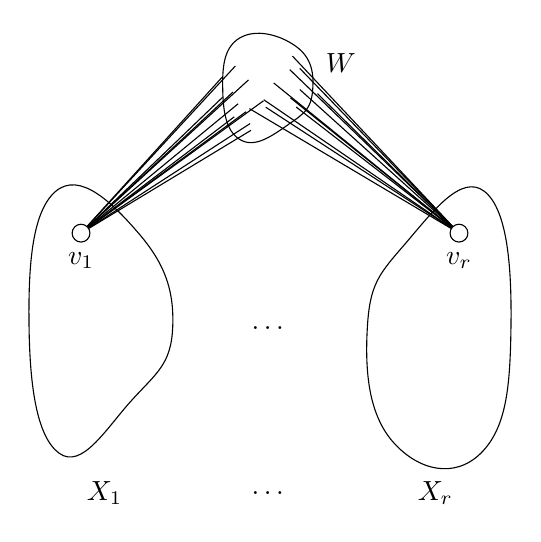
\begin{tikzpicture}[scale=0.6]
            \node [node,label=below:$v_1$] (a) at ( -4,  2) {};
            \node [node,label=below:$v_r$] (b) at (  4,  2) {};

            \foreach \theta in {10, 8, ..., -10}{
                \pgfmathsetmacro\randb{rand}
                \pgfmathsetmacro\randd{rand}

                \draw  (a) -- ++(\theta*0.8 + \randb*1.4 +  40 : 4.5 + \randb*0.5);
                \draw  (b) -- ++(\theta*0.8 + \randd*1.4 + 140 : 4.7 + \randd*0.5);
            }

            \draw plot [smooth cycle, tension=0.8, yshift=5cm] coordinates {(-180:1.0) (-120:1.2) (-60:0.8) (0:0.9) (60:1.1) (120:1.3)};
            \draw plot [smooth cycle, tension=0.8, xshift=-3.5cm, yscale=1.6, scale=1.6] coordinates {(-180:1.0) (-120:1.2) (-60:0.7) (0:0.9) (60:0.9) (120:1.3)};
            \draw plot [smooth cycle, tension=0.8, xshift=3.5cm, yscale=1.6, scale=-1.6] coordinates {(-180:1.0) (-120:1.3) (-60:0.8) (0:0.9) (60:1.1) (120:1.2)};

            \node at (1.5,5.6) {$W$};
            \node at (-3.5, -3.5) {$X_1$};
            \node at (0, -3.5) {$\dots$};
            \node at (0, 0) {$\dots$};
            \node at (3.5, -3.5) {$X_r$};
        \end{tikzpicture}
    \end{center}
    Let
    \begin{align*}
        A = \Set{(W, v_1, \dotsc, v_r) | W \subset V(G), \abs{W} = t, \forall i\ v_i \in X_i, \forall i \forall w \in W: v_i \sim w}
    \end{align*}

    What can we say about $\abs{A}$?
    First, given $v_1 \in X, \dotsc, v_r \in X_r$, we can check from the minimum degree condition that
    \begin{equation*}
        \abs{\Gamma(v_1) \cap \dotsc \cap \Gamma(v_r)} \geq r \epsilon n
    \end{equation*}
    So there are at least $\binom{r \epsilon n}{t}$ choices for $W$. Hence $\abs{A} \geq T^r \binom{r \epsilon n}{t}$.

    On the other hand given the set $W$, as $K_{r+1}(t) \not\subset G$, we know that there is some $X_i$ containing at most $t-1$ vertices joined to all of $W$.
    Hence $\abs{A} \leq \binom{n}{t} (t-1) T^{r-1}$, thus
    \begin{equation*}
        T^r \binom{r \epsilon n}{t} \leq \binom{n}{t} (t-1) T^{r-1}.
    \end{equation*}
    Now,
    \begin{equation*}
        \text{RHS} \leq \frac{n^t}{t!} (t-1) T^{r-1}
    \end{equation*}
    while
    \begin{equation*}
        \text{LHS} \geq T^r \frac{1}{t!} (r \epsilon n - t)^t \geq T^r \frac{1}{t!} \left(\frac{r \epsilon n}{2}\right)^t.
    \end{equation*}
    Combining, we get
    \begin{equation*}
        T^r \left(\frac{r \epsilon n}{2}\right)^t \leq n^t (t-1) T^{r-1}
    \end{equation*}
    hence $T \leq (\frac{2}{r \epsilon})^t (t-1)$, a contradiction.
\end{proof}
\subsection{Hamiltonian graphs}









\begin{nthm}[Dirac's Theorem]\label{thm:17}
    Let $\abs{G} = n \geq 3$ and $\delta(G) \geq \frac{n}{2}$. Then $G$ is Hamiltonian.
\end{nthm}

\begin{proof}
    First, observe $G$ is connected.
    Indeed, if $x \neq y$, $x \nsim y$, then $\abs{\Gamma(x) \cup \Gamma(y)} \leq n-2$, but $\abs{\Gamma(x)} + \abs{\Gamma(y)} \geq \frac{n}{2} + \frac{n}{2} = n$ so $\Gamma(x) \cap \Gamma(y) \neq \emptyset$.

    Let $v_0, v_1, \dotsc, v_k$ be a path of maximal length in $G$, say length $k \leq n-1$.
    By maximality, $\Gamma(v_0) \subset \{v_1, \dotsc, v_k\}$. Similarly, $\Gamma(v_k) \subset \{v_0, \dotsc, v_{k-1}\}$.
    \begin{center}
        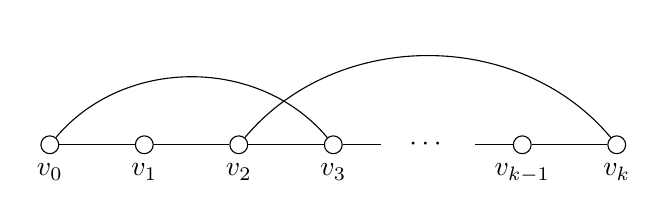
\begin{tikzpicture}[scale=1.2]
            \node [node, label=below:$v_0$]     (0) at (  0,  0)  {};
            \node [node, label=below:$v_1$]     (1) at (  1,  0)  {};
            \node [node, label=below:$v_2$]     (2) at (  2,  0)  {};
            \node [node, label=below:$v_3$]     (3) at (  3,  0)  {};

            \node [node, label=below:$v_{k-1}$] (4) at (  5,  0)  {};
            \node [node, label=below:$v_k$]     (5) at (  6,  0)  {};

            \node [draw=none] at (4, 0) {$\cdots$};
            \draw (0) -- (1) -- (2) -- (3) -- (3.5, 0);
            \draw (4.5, 0) -- (4) -- (5);
            \draw (0) to[bend left=50] (3);
            \draw (2) to[bend left=50] (5);
        \end{tikzpicture}
    \end{center}

    If we have some situation like in the diagram, we get a cycle. To be more precise, if
    \begin{equation*}
        A = \set{i \in [k] | v_0 \sim v_i} \quad \text{and} \quad B = \set{i \in [k] | v_k \sim v_{i-1}}
    \end{equation*}
    then $A \cap B \neq \emptyset \implies$ we have a cycle.
    But $\abs{A \cup B} \leq k < n$ while $\abs{A} + \abs{B} \geq \frac{n}{2} + \frac{n}{2} = n$.
    Hence $\exists i \in A \cap B$ so we have a cycle $C = v_0 v_1 \dotsc v_{i-1} v_k v_{k-1} \dotsc v_i v_0$ of length $k+1$.

    If $k = n-1$, we have a Hamiltonian cycle as required.
    If $k < n-1$, relabel the cycle $C = u_0 u_1 \dotsc u_k u_0$.
    By connectedness, we have some $u_i \in C$ and $w \notin C$ with $w \sim u_i$.
    Then $w u_i u_{i+1} \dotsc u_k u_0 \dotsc u_{i-1}$ is a path of length $k+1$, contradicting maximality.
\end{proof}







\begin{nprop}\label{thm:18}
    Let $G$ be a connected graph. Then
    \begin{equation*}
        G\text{ Eulerian if and only if } \forall v \in G,\ d(v)\text{ is even.}
    \end{equation*}
\end{nprop}
\begin{proof}
    ($\Rightarrow$) is obvious: an Eulerian circuit must go in and out of a given vertex the same number of times.

    ($\Leftarrow$): use induction on $e(G)$. For $e(G) = 0$ it is clearly true.

    Consider $e(G) > 0$. Let $v_0 v_1 \dotsc v_k = C$ be a circuit in $G$ of maximal length.
    If $C$ uses all edges of $G$ then we are done.
    If not, delete all edges used in $C$ from $G$ to form $H$.
    In $H$, every vertex still has even degree. Let $H_1$ be a component of $H$ with at least one edge.

    By induction hypothesis, $H_1$ has an Euler circuit $D$.
    Certainly $C, D$ meet at some vertex $v$.
    Join them at $v$ to produce a longer circuit in $G$, a contradiction.
    (Walk along $C$ until we get to $v$, then walk all round $D$ starting/ending at $v$, then walk along the rest of $C$).
\end{proof}
\clearpage
\section{Graph Colouring}







\subsection{Planar Graphs}










\begin{nthm}[Kuratowski's Theorem]\label{thm:19}
    Let $G$ be a graph. Then $G$ planar iff $G$ contains no subdivision of $K_5$ or $K_{3,3}$.
\end{nthm}





\begin{nprop}\label{prop:20}
    Every tree of order at least $2$ has a leaf.
\end{nprop}
\begin{proof}
    Let $T$ be a tree $\abs{T} \geq 2$ and let $v_0 v_1 \dotsc v_k$ be a path of maximum length in $T$.
    Now $v_k \sim v_{k-1}$, but $v_k$ has no other neighbours in the path (as $T$ acyclic) and $v_k$ has no neighbours outside path (by maximality).
    Hence $v_k$ is a leaf.
\end{proof}







\begin{nprop}\label{prop:21}
    Let $T$ be a tree, $\abs{T} = n \geq 1$. Then $e(T) = n-1$.
\end{nprop}
\begin{proof}
    Use induction on $n$. For $n=1$, $e(T) = 0$ as required.

    For $n > 1$, let $v$ be a leaf.
    Then $T - v$ is a tree with $\abs{T - v} = n-1$ so by the induction hypothesis, $e(T-v) = n-2$, so $e(T) = n-1$.
\end{proof}
\begin{nprop}\label{prop:22}
    Every tree is planar.
\end{nprop}
\begin{proof}
    Let $T$ be a tree, $\abs{T} = n$ and use induction on $n$.
    For $n=0,1$ we are done immediately.

    For $n > 1$, let $v \in T$ be a leaf.
    By the induction hypothesis, $T-v$ can be drawn.
    Let $u \in T$ be the neighbour of $v$.
    Take a small circle around $u$ in the drawing; so the circle contains only the centre and some radii in the drawing.
    Hence, we can easily add $v$ and $uv$ to the drawing.
\end{proof}


\begin{nthm}[Euler's Formula]\label{thm:23}
    Take $G$ connected and planar.
    Take $\abs{G} = n \geq 1$, $e(G) = m$ with $l$ faces.
    Then $n - m + l = 2$.
\end{nthm}
\begin{proof}
    Induction on $m$. If $G$ is a tree: $m = n-1$, $l = 1$, and we are done.

    Otherwise, $G$ has a cycle.
    Pick an edge $e$ in the cycle and consider $G-e$. Then $\abs{G - e} = n$, $e(G-e) = m-1$.
    Moreover, in our drawing, removing $e$ combines two faces so we have drawn $G-e$ with $l-1$ faces.
    So, by the induction hypothesis $n - (m-1) + (l-1) = 2$, so $n - m + l = 2$.
\end{proof}
\begin{ncor}\label{cor:24}
    Let $G$ be planar, $\abs{G} = n \geq 3$. Then $e(G) \leq 3n-6$.
\end{ncor}
\begin{proof}
    Let $e(G) = m$. Draw $G$ with $l$ faces.
    Without loss of generality, $G$ is connected (if not, add edges to make it so).

    We have a special case where
    \begin{center}
        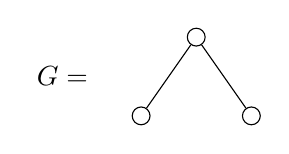
\begin{tikzpicture}
            \node at (-1,0) {$G=$};
            \node [node] (A) at (0  ,-0.5) {};
            \node [node] (B) at (0.7, 0.5) {};
            \node [node] (C) at (1.4,-0.5) {};
            \draw (A) -- (B) -- (C);
        \end{tikzpicture}
    \end{center}
    with $n = 3$, $m = 2$ and $3n-6 = 3 \geq 2$.

    Otherwise, we know $n - m + l = 2$ and each face has at least 3 edges in its boundary, and each edge is in the boundary of at most 2 faces.
    So, $l \leq \frac{2m}{3}$.
    Thus, $n -m + \frac{2}{3}m \geq 2$ so $\frac{1}{3}m \geq n-2$ so $m \geq 3n-6.$
\end{proof}
\begin{nprop}[Six colour theorem]\label{prop:25}
    Any planar graph is 6-colourable.
\end{nprop}
\begin{proof}
    Let $G$ be planar, $\abs{G} = n$. Induction on $n$.
    For $n \leq 6$, give every vertex a different colour, as required.

    For $n > 6$, by \cref{cor:24}, $e(G) \leq 3n - 6$. Hence
    \begin{equation*}
        \delta(G) \leq \frac{2 e(G)}{\abs{G}} \leq \frac{6n-12}{n} = 6 - \frac{12}{n} < 6.
    \end{equation*}
    So, $\delta(G) \leq 5$.

    Pick $v \in G$ with $d(v) \leq 5$. By inductive hypothesis, $G- v$ can be 6-coloured.
    Some colour is missing from $\Gamma(v)$, use this colour to colour $v$.
\end{proof}
\begin{nthm}[Five colour theorem]\label{thm:26}
    Any planar graph is 5-colourable.
\end{nthm}
\begin{proof}
    Let $G$ be planar, $\abs{G} = n$.
    Use induction on $n$.
    The base case $n\leq 5$ is trivial, so take $n > 5$.
    As in \cref{prop:25}, we can find $v \in G$ with $\delta(v) \leq 5$ and 5-colour $G-v$.
    If there is a colour missing from $\Gamma(v)$, use that colour at $v$.
    Otherwise, draw $G$; WLOG $v$ has neighbours $x_1, \dotsc, x_5$ in clockwise order around $v$ with colours $\green{1}, \red{2},\purple{3},\blue{4},\orange{5}$ respectively.

    \hypertarget{def:ijpath}Call a path in $G-v$ an \textbf{$ij$-path} if all its vertices have colour $i$ or $j$.
    \hypertarget{def:ijcomp}Given $x \in G-v$, the \textbf{$ij$-component} of $x$ consists of those vertices reachable from $x$ along $ij$-paths.

    If $x_1, x_3$ are in different $\green{1}\purple{3}$ components, then swap the colours of $1,3$ on the $\green{1}\purple{3}$ component of $x_1$ and give $v$ colour $\green{1}$.
    \begin{center}
        \begin{tikzpicture}[scale=2]
            \node [node,thick,        label=below:$v$]   (v) at (0,0)  {};
            \node [node,thick,bgreen   ,label=above:$x_1$] (x1) at ( 90:1) {};
            \node [node,thick,bred,label=right:$x_2$] (x2) at ( 18:1) {};
            \node [node,thick,bpurple  ,label=below:$x_3$] (x3) at (-54:1) {};
            \node [node,thick,bblue,label=below:$x_4$] (x4) at (-126:1) {};
            \node [node,thick,borange ,label=left :$x_5$] (x5) at (162:1) {};
            \begin{scope}[every node/.style={node,thick}]
                \node [bpurple] (y1) at (1,1.4) {};
                \node [bgreen]    (y2) at (2,1) {};
                \node [bpurple] (y3) at (2.1,0) {};
                \node [bgreen]    (y4) at (1.6,-0.8) {};
            \end{scope}
            \foreach \x in {1,...,5} { \draw (v) -- (x\x); }
            \draw (x1) -- (y1) -- (y2) -- (y3) -- (y4) -- (x3);
        \end{tikzpicture}
    \end{center}

    If not, then $x_2, x_4$ are in different $\red{2}\blue{4}$ components as we see in the diagram, so swap colours $2, 4$ on the $\red{2}\blue{4}$ component of $x_2$ and give $v$ colour $\red{2}$.
\end{proof}
\begin{nthm}[Four colour theorem]\label{thm:27}
    Any planar graph is 4-colourable.
\end{nthm}
\begin{proof}
    Let $G$ be planar, $\abs{G} = n$ and use induction on $n$. For $n=4$, we are immediately done.

    For $n > 4$, pick $v \in G$ with $d(v) \leq 5$, then draw $G$ and 4-colour $G-v$.
    If some colour is missing on $\Gamma(v)$ then we are done.
    If not, there are three cases.

    Case 1: $d(v) = 4$.
    There cannot be both a $\green{1}\purple{3}$-path from $x_1$ to $x_3$ and a $\red{2}\blue{4}$ path from $x_2$ to $x_4$, so done as in the proof of \cref{thm:26}.
    \begin{center}
        \begin{tikzpicture}[scale=2]
            \node [node,thick]   (v) at (0,0)  {};
            \node (x1) at (0,1) {};
            \node (x3) at (0,-1) {};
            \node [node,thick,bred,label=right:$x_2$] (x2) at (1,0) {};
            \node [node,thick,bblue,label=below:$x_4$] (x4) at (-1,0) {};
            \foreach \x in {1,...,4} {
                \draw (v) -- (x\x);
            }
            \draw plot [smooth, tension=1.6] coordinates {(x1) (2,0) (x3)};
            \node [node,thick,bgreen,fill=white,label=above:$x_1$] at (x1)  {};
            \node [node,thick,bpurple,fill=white,label=below:$x_3$] at (x3) {};
            \draw [->] (x2) to [bend left=10] (0.6,-0.4);
            \node at (0.5,-0.5) {$\times$};
        \end{tikzpicture}
    \end{center}

    Case 2: $d(v) = 5$, $v$ has neighbours $x_1, \dotsc, x_5$ clockwise with colours $\green{1},\red{2},\purple{3},\blue{4},\green{1}$.

    \begin{center}
        \begin{tikzpicture}[scale=2]
            \node [node,thick] (v) at (0,0) {};
            \node (x1) at ( 0.6,0.9) {};
            \node (x5) at (-0.6,0.9) {};
            \node (x2) at (1,0) {};
            \node (x3) at (0,-1) {};
            \node (x4) at (-1,0) {};
            \foreach \x in {1,...,5} {
                \draw (v) -- (x\x);
            }
            \draw plot [smooth, tension=1.6] coordinates {(x2) (0,-1.5) (x4)};
            \node [node,thick,bgreen, fill=white,label=above:$x_1$] at (x1) {};
            \node [node,thick,bgreen, fill=white,label=above:$x_5$] at (x5) {};
            \node [node,thick,bpurple,fill=white,label=below:$x_3$] at (x3) {};
            \node [node,thick,bred,   fill=white,label=right:$x_2$] at (x2) {};
            \node [node,thick,bblue,  fill=white,label=left :$x_4$] at (x4) {};
            \draw [->] (x3) to [bend left=10] (-0.4,-0.6);
            \node at (-0.5,-0.5) {$\times$};
        \end{tikzpicture}
    \end{center}
    Then there is either no $\red{2}\blue{4}$ path from $x_2$ to $x_4$ or no $\green{1}\purple{3}$ path from $x_3$ to $x_1$, so again we are done.

    Case 3: $d(v) = 5$, colours $\green{1},\red{2},\purple{3},\green{1},\blue{4}$.
    \begin{center}
        \begin{tikzpicture}[scale=2]
            \node [node,thick] (v) at (0,0) {};
            \node (x1) at (54:1) {};
            \node (x2) at (-18:1) {};
            \node (x3) at (-90:1) {};
            \node (x4) at (-162:1) {};
            \node (x5) at (126:1) {};
            \foreach \x in {1,...,5} {
                \draw (v) -- (x\x);
            }
            \draw plot [smooth, tension=1.6] coordinates {(x2) (54:1.5) (x5)};
            \draw plot [smooth, tension=1.6] coordinates {(x5) (-162:1.5) (x3)};

            \node [node,thick,bgreen, fill=white,label=above:$x_1$] at (x1) {};
            \node [node,thick,bred,   fill=white,label=right:$x_2$] at (x2) {};
            \node [node,thick,bpurple,fill=white,label=below:$x_3$] at (x3) {};
            \node [node,thick,bgreen, fill=white,label=left :$x_4$] at (x4) {};
            \node [node,thick,bblue,  fill=white,label=above:$x_5$] at (x5) {};
        \end{tikzpicture}
    \end{center}
    If there is no $\red{2}\blue{4}$ path from $x_2$ to $x_5$, we are done.
    If there is no $\purple{3}\blue{4}$ path from $x_3$ to $x_5$, we are done.

    Otherwise, swap colours $\green{1},\purple{3}$ on the $\green{1}\purple{3}$ component of $x_1$ and swap colours $\green{1},\red{2}$ on the $\green{1}\red{2}$ component of $x_4$.
    Then, use colour $\green{1}$ at $v$, but this is false.
\end{proof}
% new lec


\subsection{General Graphs}









{
}


{
}















\begin{nthm}[Brooks' theorem]\label{thm:28}
    Let $G$ be a connected graph that is neither complete nor an odd cycle.
    Then $\chi(G) \leq \Delta(G)$.
\end{nthm}
\begin{proof}
    Induction on $|G|$. Write $\Delta = \Delta(G)$.
    We cannot have $\Delta = 0,1$ as $G \ncong K_1, K_2$.
    If $\Delta = 2$ then $G$ is a path or an even cycle, so $\chi(G) = 2$.
    So assume $\Delta \geq 3$. Pick $v \in G$ and let $H$ be a component of $G - v$.

    \textbf{Either} $\Delta(H) < \Delta$, in which case by greedy algorithm bound \eqref{eq:greedystar} we have \begin{equation*}\chi(H) \leq \Delta(H) + 1 \leq \Delta.\end{equation*}
    \textbf{Or} $\Delta(H) = \Delta$. Then $H$ is connected and not an odd cycle (as $\Delta \geq 3$).
    Moreover, $\exists u \in H$ with $u \sim v$ in $G$.
    In $G$, $d(u) \leq \Delta$ so in $H$, $d(u) \leq \Delta - 1$.
    So $H$ is not regular, so not complete.
    Hence by induction hypothesis, $\chi(H) \leq \Delta$.

    Do this for each component of $G - v$ to obtain a $\Delta$-colouring $c$ of $G - v$.
    If there is a colour missing from $\Gamma(v)$, then use that colour at $v$, as required.
    So assume that is not the case.

    So have $\Gamma(v) = \{x_1, \dotsc, x_\Delta\}$ with $\forall i, c(x_i) = i$.
    We can also assume:
    \begin{enumerate}[label=(\roman*)]
        \item if $i \neq j$ then there is an $ij$-path $P_{ij}$ from $x_i$ to $x_j$,
        \item if $i \neq j$ then $P_{ij}$ is entire $ij$-component containing $x_i,x_j$, and
        \item if $i, j, k$ distinct then $P_{ij}, P_{ik}$ meet only at $x_i$.
    \end{enumerate}
    (Why? If any of these fail then it is easy to check that the colouring $c$ can be modified to change the colour of $x_i$ and allowing us to use colour $i$ at $v$).
    \begin{enumerate}[label=(\roman*)]
        \item is as in previous proofs.
        \item if $P_{\red{i}\green{j}}$ is not the entire $\red{i}\green{j}$-component, then
            at some point in the path we get a point (wlog colour \green{$j$}) which `branches off'.
            \begin{center}
                \begin{tikzpicture}
                    \node [node,       thick] (v) at (0,0) {};
                    \node [node,bgreen,thick] (j) at (0.2,1) {};
                    \node [node,bred,  thick] (i) at (1,-0.2) {};
                    \draw[path fading=west] (v) -- ( 170:1);
                    \draw[path fading=west] (v) -- (-160:1);
                    \draw[path fading=west] (v) -- (-140:1);
                    \draw[path fading=west] (v) -- (-130:1);
                    \draw[path fading=south] (v) -- ( -96:1);

                    \draw (j) -- (v) -- (i);
                    \node [node, bred,   thick] (i2) at (1.2,1.1) {};
                    \node [node, bgreen, thick] (j2) at (1.7,0.4) {};
                    \node [node, bgreen, thick] (j3) at (1.8,1.7) {};

                    \draw (j) -- (i2) -- (j3);
                    \draw (i2) -- (j2) -- (i);
                \end{tikzpicture}
            \end{center}
            Then this vertex has 3 \green{green} neighbours, so there are at most $\Delta - 3$ colours used in the rest of its neighbours, so there is a colour not in the colours of its neighbours$\cup \{i,j\}$.
            We can swap it to that, breaking the chain $P_{ij}$.
        \item if $P_{ij}, P_{ik}$ meet at some point which must have colour $i$, then that point has 2 $j$ neighbours and 2 $k$ neighbours, so as before there is a colour other than $i$ that none of its neighbours have, which we can swap it to, breaking $P_{ij}$ and $P_{ik}$.
    \end{enumerate}

    As $G \ncong K_{\Delta+1}$, there are some $i, j$ with $i \neq j$, $x_i \nsim x_j$.
    As $\Delta \geq 3$, pick $k \in [\Delta] \setminus \{i, j\}$.
    Let $u$ be the neighbour of $x_i$ of colour $j$.
    Swap colours $i,k$ on the $ik$-component of $x_i$ (i.e.\ on $P_{ik}$).
    This gives a new colouring $c'$, with $c'(x_i) = k$, $c'(x_k) = i$.

    Also, if $w \in P_{ij}$ with $w \neq x_i$ then $c'(w) = c(w)$ so $c'(x_j)=c'(u) = j$.
    $c'$ must satisfy conditions (i),(ii),(iii) as before.
    Then by (i) there is a $kj$-path from $x_i$ to $x_j$ , $P'_{kj}$ .
    By (ii), $u \in P'_{kj}$.

    By (i), there is a $ji$-path $P'_{ji}$ from $x_j$ to $x_k$.
    By (ii), $u \in P'_{ji}$.
    But now $P'_{kj}$ and $P'_{ji}$ meet at $u$, contradicting (iii).
\end{proof}
\subsection{Graphs on surfaces}






















\begin{nthm}[Heawood's Theorem]\label{thm:29}
    Let $S$ be a closed boundaryless surface of Euler characteristic $E \leq 1$. Then
    \begin{equation*}
        \chi(S) \leq \floor*{\frac{7 + \sqrt{49-24E}}{2}}.
    \end{equation*}
\end{nthm}
\begin{proof}
    Let $\chi = \chi(S)$. Let $G$ be a minimal $\chi$-colourable graph that can be drawn on $S$ - i.e.\ $\chi(G) = \chi$ but
    \begin{equation*}H \subset G, H \neq G \implies \chi(G) \leq \chi - 1.\end{equation*}
    Clearly $G$ is connected and $|G| \geq \chi$.

    Let $|G| = n \geq \chi$, $e(G) = m$ and draw $G$ on $S$ with $l$ faces.
    Then by Euler-Poincar\'e, $n - m + l \geq E$.
    As before, $l \leq \frac{2}{3} m$ so $n - \frac 13 m \geq E$ so $m \leq 3n - 3E$.
    Hence
    \begin{equation*}
        \delta(G) \leq \frac{2m}{n} \leq \frac{6n-6E}{n} = 6 - \frac{6E}{n}. \tag{$*$} \label{eq:heawoodstar}
    \end{equation*}
    On the other hand, if $v \in G$ then $G - v$ is $(\chi-1)$-colourable and this colouring does not extend to a $(\chi-1)$-colouring of $G$ so $d(v) \geq \chi-1$.
    Hence $\delta(G) \geq \chi-1$.

    Combining this with \eqref{eq:heawoodstar}:
    If $E \leq 0$: $\chi - 1 \leq \delta(G) \leq 6 - \frac{6E}{n} \leq 6 - \frac{6E}{\chi}$ as $n \geq \chi$.
    Hence $\chi^2 - 7\chi + 6E \leq 0$ and so $\chi \leq \frac{7 + \sqrt{49 + 24 E}}{2}$.

    If $E = 1$, $\delta(G) \leq 6 - \frac{6}{n} < 6$ so $\delta(G) \leq 5$. Hence $\chi-1 = 5$ so $\chi \leq 6 = \frac{7 + \sqrt{49 + 24}}{2}$.
\end{proof}




























\subsection{Edge Colouring}




\begin{nthm}[Vizing's theorem]\label{thm:30}
    Let $G$ be a graph. Then
    \begin{equation*}
        \chi'(G) \leq \Delta(G) + 1
    \end{equation*}
\end{nthm}
\begin{proof}
    Induction on $e(G)$. The $e(G) = 0$ case is immediate.

    For $e(G) > 0$, let $\Delta = \Delta(G)$. Pick an edge $xy$.
    By the induction hypothesis we can find an $(\Delta+1)$-edge colouring of $G - x y_1$, call it $\varphi$.

    As $\Delta(G) < \Delta + 1$, there some colour `missing' at each vertex.
    Let $c_1$ be missing at $y_1$. If $c_1$ is also missing at $x$, then colour $xy_1$ with colour $c$, so done.

    If not, let $y_2 \in \Gamma(x)$ with $\varphi(x y_2) = c_1$ and let $c_2$ be missing at $y_2$.
    % possible pic missing
    Continue inductively ($*$):
    Given distinct $y_1, \dotsc, y_n \in \Gamma(x)$, distinct colours $c_1, \dotsc, c_k$ such that $c_i$ is missing at $y_i$ (for $1 \leq i \leq k$) and $\varphi(x y_{i+1}) = c_i$ (for $1 \leq i \leq k-1$).
    If $c_k$ is missing at $x$, re-colour $xy_i$ in colour $c_i$.
    Otherwise, let $y_{k+1} \in \Gamma(x)$ with $\varphi(x y_{k+1}) = c_k$.
    Let $c_{k+1}$ be missing at $y_k$. If $c_{k+1} \notin \{c_1, \dotsc, c_k\}$, continue as at ($*$).

    Otherwise assume WLOG $c_{k+1} = c_1$. (If instead $c_{k+1} = c_j$ for some $j > 1$, then uncolour $xy_j$, recolour $x y_i$ in colour $c_i$ for $1 \leq i < j$ and relabel $y_j, y_{j+1}, \dotsc$ as $y_1, y_2, \dotsc$).
    Let $c$ be a colour missing at $x$.
    Consider the $cc_1$ subgraph of $G$, i.e.\ only edges coloured $c$ or $c_1$.
    This subgraph has maximum degree $\leq 2$ so each component is a path or a cycle.
    Moreover, $x,y_1,y_{k+1}$ have degree $\leq 1$ in this subgraph so $x_1, y_1, y_{k+1}$ are not all in the same component.

    If $x,y_1$ in different $c c_1$ component, then swap $c,c_1$ on the component of $y_1$ and give $x y_1$ colour $c$.
    Otherwise $x, y_{k+1}$ in different components. In this case, uncolour $x y_{k+1}$ and recolour $x y_i$ with colour $c_i$ for $1 \leq i \leq k$.
    Then swap colours $c,c_1$ on the $c c_1$-component of $y_{k+1}$ and give $x y_{k+1}$ colour $c$.
\end{proof}
\clearpage
\section{Connectivity}
\subsection{The Marriage Problem}















\begin{nthm}[Hall's Marriage Theorem]\label{thm:31}
    Let $G$ be a bipartite graph with bipartition $(X,Y)$.
    Then $G$ has a matching from $X$ to $Y$ iff $G$ satisfies \textbf{Hall's condition}:
    \begin{equation*}
        \hypertarget{def:hall}\forall A \subset X, \abs{\Gamma(A)} \geq |A|
    \end{equation*}
\end{nthm}
\begin{proof}
    $(\Rightarrow)$ is obvious. For $(\Leftarrow)$, use induction on $|X|$.
    $|X|=0,1$ are immediate.

    For $|X|\geq 2$, there are two cases. The easy case has $|\Gamma(A)| > |A|$ for all $A \subset X$ with $A \neq \emptyset,X$.
    Pick any $x \in X$. $|\Gamma(x)| \geq 1$ so pick $y \in \Gamma(x)$.
    Look at $G - \{x,y\}$; this graph satisfies Hall's condition, so has a matching from $X - \{x\}$ to $Y - \{y\}$. Add edge $xy$, and done.

    The harder case has $|\Gamma(A)| = |A|$ for some $A \neq 0,X$.
    Let
    \begin{align*}
        G_1 &= G[A \cup \Gamma(A)] \\
        G_2 &= G[(X \setminus A) \cup (Y \setminus \Gamma(A))].
    \end{align*}
    \begin{center}
        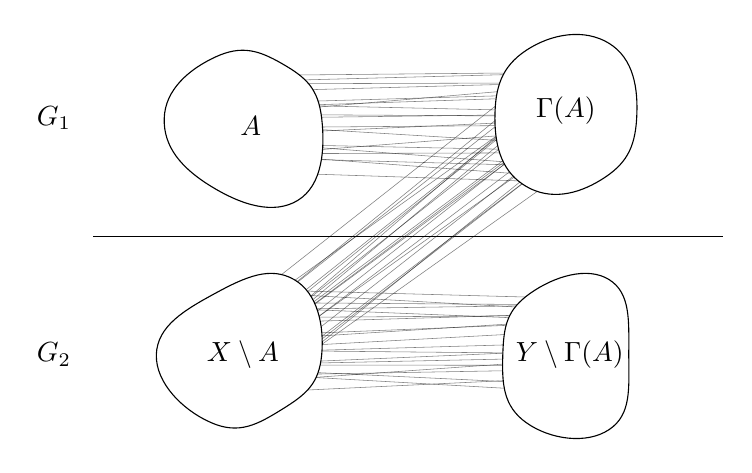
\begin{tikzpicture}
            \foreach \x in {1,...,20} {
                \draw[very thin,opacity=0.5] (0,2.25+\x/15+rand*0.2) -- (4,2.25+\x/15+rand*0.2);
                \draw[very thin,opacity=0.5] (0,-0.7+\x/15+rand*0.2) -- (4,2.4+\x/15+rand*0.2);
                \draw[very thin,opacity=0.5] (0,-0.5+\x/15+rand*0.2) -- (4,-0.5+\x/15+rand*0.2);
            }
            \draw[fill=white] plot [smooth cycle, tension=0.8]                       coordinates {(-180:1.2) (-120:1) (-60:0.8) (0:0.9) (60:1.1) (120:0.9)};
            \draw[fill=white] plot [smooth cycle, xshift=4cm, tension=0.8]           coordinates {(-180:0.8) (-120:1) (-60:1.1) (0:0.8) (60:1.1) (120:0.9)};
            \draw[fill=white] plot [smooth cycle, yshift=3cm, tension=0.8]           coordinates {(-180:1.1) (-120:1) (-60:1.2) (0:0.9) (60:0.8) (120:0.9)};
            \draw[fill=white] plot [smooth cycle, xshift=4cm,yshift=3cm,tension=0.8] coordinates {(-180:0.9) (-120:1) (-60:0.9) (0:0.9) (60:1.1) (120:1.0)};
            \node at (-2.5,3) {$G_1$};
            \node at (-2.5,0) {$G_2$};
            \node at (-0.1,0) {$X\setminus A$};
            \node at (0,2.9) {$A$};
            \node at (4,3.1) {$\Gamma(A)$};
            \node at (4.05,0) {$Y\setminus\Gamma(A)$};
            \draw (-2,1.5) -- (6,1.5);
        \end{tikzpicture}
    \end{center}
    First, $G_1$ obviously satisfies Hall's condition so $\exists$ a matching $A$ to $\Gamma(A)$.
    What about $G_2$? Take $B \subset X \setminus A$.
    Then
    \begin{equation*}|\Gamma_{G_2}(B)| = |\Gamma(A\cup B)\setminus \Gamma(A)| = |\Gamma(A \cup B)| - |\Gamma(A)| \geq |A \cup B| - |A|=|B|.\end{equation*}
    Hence $G_2$ also satisfies Hall and has a matching from $X \setminus A$ to $Y \setminus \Gamma(A)$.
    Combine the two matchings to get a matching from $X$ to $Y$ in $G$.
\end{proof}





\begin{ncor}[Defect Hall]\label{cor:32}
    Let $G$ be a bipartite graph with bipartition $(X,Y)$ and let $d \geq 1$.
    Then $G$ contains $|X|-d$ independent edges if and only if $\forall A \subset X, \ |\Gamma(A)| \geq |A| - d$.
\end{ncor}
\begin{proof}
    ($\Rightarrow$) is immediate.
    ($\Leftarrow$). In marriage terminology: Introduce $d$ imaginary perfect men, suitable husbands for all the women.
    This satisfies Hall's condition so has matching from $X$ to $Y$.
    In real life, at most $d$ women unmarried.
\end{proof}
\begin{ncor}[Polyandrous Hall]\label{cor:33}
    Let $G$ be a bipartite graph, bipartition $(X,Y)$, $d \geq 2$.
    Then $G$ contains a set of $d |X|$ edges, each vertex in $X$ in precisely $d$ of them, each vertex in $Y$ in at most one $\iff \forall A \subset X, |\Gamma(A)| \geq d |A|$.
\end{ncor}
\begin{proof}
    ($\Rightarrow$) is immediate.
    ($\Leftarrow$). In marriage terminology: clone each woman $d-1$ times so there are $d$ copies of each.
    This satisfies Hall's condition so have matching from $X$ to $Y$.
    Destroy the clones.
\end{proof}


\subsection{Connectivity}
























\begin{nthm}\label{thm:34}
    Let $G$ be a graph and $A,B \subset V(G)$.
    Let
    \begin{equation*}
        k = \min \set{\abs{W} | W \text{ is an $AB$-separator}}.
    \end{equation*}
    Then $G$ contains $k$ vertex-disjoint $AB$-paths.
\end{nthm}




\begin{proof}
    Coming soon.
\end{proof}
\begin{ncor}[Menger's Theorem]\label{cor:35}
    Let $G$ be an incomplete $k$-connected graph and let $a,b \in V(G)$, $a \neq b$.
    Then $G$ contains $k$ independent $ab$-paths.
\end{ncor}
\begin{proof}
    Suppose first $a \nsim b$. Let $A = \Gamma(a)$ and $B = \Gamma(b)$.
    We have $G$ $k$-connected and $G-A,G-B$ disconnected, so $|A|,|B|\geq k$.

    Hence, any $AB$-separator $W$ has $|W| \geq k$, so by \Cref{thm:34}, there are $k$ vertex-disjoint $AB$ paths.
    Extend these to $a$,$b$.

    If instead $a \sim b$: $G-ab$ is $(k-1)$-connected, so has $k-1$ independent $ab$ paths by first part.
    $ab$ is another, as required.
\end{proof}











\begin{proof}[Proof of \Cref{thm:34}]
    Induction on $e(G)$.
    If $e(G) = 0$, the smallest $AB$-separator is $A \cap B$, and each vertex of $A \cap B$ gives an $AB$-path (of length zero), so done.

    If $e(G) > 0$, pick $xy \in E(G)$.
    Let $W$ be an $AB$-separator of minimum order in $G - xy$.
    If $|W| \geq k$ then by the induction hypothesis there are $k$ vertex-disjoint $AB$-paths in $G-xy$ and so also in $G$.

    So assume $|W| < k$. Then $W \cup \{x\}$ is an $AB$-separator in $G$.
    Hence $|W \cup \{x\}| \geq k$ so $|W| \geq k-1$ so $|W| = k-1$.
    Write $W = \{w_1, w_2, \dotsc, w_{k-1}\}$. As $|W| < k$, $G-W$ contains an $AB$-path.
    This path must include the edge $xy$.
    Assume WLOG $x$ comes before $y$ in this path (if not, swap $x$ and $y$).

    Let $X = W \cup \{x\}$ and $Y = W \cup \{y\}$.
    Let $U$ be an $AX$-separator in $G-xy$. Then $U$ is an $AB$-separator in $G$, so $|U| \geq k$.
    So by the induction hypothesis, we have $k$ vertex-disjoint $AX$-paths in $G-xy$, say $P_0, P_1, \dotsc, P_{k-1}$ ending at $x, w_1, \dotsc, w_{k-1}$ respectively.

    Similarly, there are $k$ vertex-disjoint $YB$ paths in $G-xy$, say $Q_0, Q_1, \dotsc, Q_{k-1}$ starting at $y, w_1, w_2, \dotsc, w_{k-1}$ respectively.

    Given path $P=u_0 u_1 \dotsm u_l$ and $Q = v_0 v_1 \dotsm v_m$ meeting only at $u_l = v_0$, write $P \vee Q$ for the path $u_0 \dotsm u_l v_1 \dotsm v_m$.
    Then $P_0 \vee xy \vee Q_)$ and $P_i \vee Q_i$ (for $1 \leq i \leq k-1$) are $k$ vertex-disjoint $AB$-paths in $G$.
\end{proof}


















\subsection{Edge connectivity}

\begin{ncor}[Edge Menger]\label{cor:36}
    Let $G$ be $l$-edge connected and $a,b \in V(G)$ be distinct.
    Then $G$ has $l$ edge-disjoint $ab$-paths.
\end{ncor}
\begin{proof}
    The \hypertarget{def:linegraph}{\textbf{line graph}} of $G=(V,E)$ is the graph $L(G) = (E,F)$ where
    \begin{equation*}
        F = \set{ee' | e,e' \in E,\ e,e' \text{ share precisely one vertex}}.
    \end{equation*}
    Then $L(G)$ is $l$-connected.
    Add extra vertices $a',b'$ to $L(G)$ with
    \begin{itemize}
        \item $a'$ joined to each $e \in E$ with $a \in e$ and
        \item $b'$ joined to each $e \in E$ with $b \in e$.
    \end{itemize}

    By \Cref{cor:35}, $L(G)$ has $l$ independent $a'b'$-paths.
    This yields $l$ edge-disjoint $ab$-paths in $G$.
\end{proof}
\clearpage
\section{Probabilistic Techniques}
\subsection{The Probabilistic Method}







\begin{nthm}[Erd\H{o}s]\label{thm:37}
    \begin{equation*}
        R(s) = \Omega(\sqrt{2}^s)
    \end{equation*}
\end{nthm}
\begin{proof}
    Fix $n,s$. Colour each edge of $K_n$ \red{red}/\green{green} at random, independently, each colour equally likely.
    Given $H \subset K_n$ with $H \cong K_s$,
    \begin{align*}
        \mathbb{P}(H\text{ monochromatic}) &= 2 \mathbb{P}(H\text{ \red{red}}) = 2 \times \left(\frac{1}{2}\right)^{\binom{s}{2}}. \\
        \shortintertext{So}
        \mathbb{P}(K_n \text{ has a monochromatic } K_5) &\leq \binom{n}{s} \cdot 2 \cdot \left(\frac{1}{2}\right)^{\binom{s}{2}}  \\
                                        &\leq \frac{n^s}{s!} \cdot 2 \left(\frac{1}{2}\right)^{\binom{s}{2}} \\
                                        &\leq n^s \cdot 2^{-\frac{s(s-1)}{2}} \\
                                        &= \left(\frac{n}{\sqrt{2}^{s-1}}\right)^s < 1 \quad \text{if $n < \sqrt{2}^{s-1}$.}
    \end{align*}
    So if $n < \sqrt{2}^{s-1}$ then there is \emph{some} colouring with no monochromatic $K_5$.
    So $R(s) \geq \sqrt{2}^{s-1}$.
\end{proof}
\subsection{Modifying a Random Graph}













\begin{nthm}\label{thm:38}
    If $t \geq 2$ then $z(n,t) = \Omega(n^{2 - \frac{2}{t+1}})$.
\end{nthm}
\begin{proof}
    Strategy: Given $n,p$, let $G$ be a random bipartite graph with vertex classes $X,Y$ with $|X|=|Y|=n$, where for each $x \in X$, $y \in Y$ we have $xy \in E(G)$ with probability $p$, independently.
    Let $A = e(G)$ and $B$ be the number of copies of $K_{t,t}$ in $G$ (so $A$,$B$ are random variables).

    Aim: Given $n$, try to choose $p$ such that $\mathbb{E}(A-B)$ is large, specifically $\mathbb{E}(A-B) = \Omega(n^{2 - \frac{2}{t+1}})$.
    Then we can find a specific graph $G$ with $A-B = \Omega(n^{2-\frac{2}{t+1}})$.
    Remove an edge from each $K_{t,t}$ in $G$ to form a graph $H$ with no $K_{t,t}$ and $e(H) = \Omega(n^{2 - \frac{2}{t+1}})$, as required.

    Now, $\mathbb{E}(A) = n^2 p$ and $\mathbb{E}(B) = \binom{n}{t}^2 p^{t^2} \leq \frac{1}{(t!)^2} n^{2t}p^{t^2}$.
    So $\mathbb{E}(A-B) \geq n^2 p - \frac{1}{t!^2} n^{2t} p^{t^2}$.

    We want $n^2 p = n^{2t} p^{t^2}$ i.e.\ $p = n^{\frac{2-2t}{t^2-1}} = n^{-\frac{2}{t+1}}$.
    So, take $p = n^{-\frac{2}{t+1}}$.
    Then
    \begin{equation*}
        \mathbb{E}(A-B) \geq \left(1 - \frac{1}{(t!)^2}\right) n^{2 - \frac{2}{t+1}}. \qedhere
    \end{equation*}
\end{proof}



\begin{nthm}\label{thm:39}
    Let $g \geq 3$, $k \geq 2$. Then there is a graph $G$ with no cycles of length $\leq g$ and $\chi(G) \geq k$.
\end{nthm}
\begin{proof}
    Strategy: Fix $n$ and $p$. Let $G$ be a random graph with $n$ vertices, each possible edge present independently with probability $p$.
    Let $X$ be the number of short cycles in $G$.
    Recall that $\chi(G) \geq \frac{|G|}{\alpha(G)}$ where $\alpha(G)$ is the independence number of $G$.
    For cycles, by `short', we mean of length $\leq g$.

    Aim: Pick $n$ and $p$ such that
    \begin{enumerate}
        \item $\mathbb{P}(X > \frac{n}{2}) < \frac{1}{2}$ and
        \item $\mathbb{P}(\alpha(G) \geq \frac{n}{2k}) > \frac{1}{2}$.
    \end{enumerate}
    Then $\mathbb{P}(X > \frac{n}{2} \text{ or } \alpha(G) \geq \frac{n}{2k}) < 1$ so can pick a specific $G$ such that $X \leq \frac{n}{2}$ and $\alpha(G) < \frac{n}{2k}$.
    Remove a vertex from each short cycle to get $H$ with $|H| \geq \frac{n}{2}$ and $\alpha(H) < \frac{n}{2k}$ so $\chi(H) > \frac{n/2}{n/(2k)} = k$, as required.

    \begin{enumerate}
        \item For $3 \leq i \leq g$, let $X_i$ be the number of cycles of length $i$ appearing as subgraphs of $G$.
            Then
            \begin{equation*}
                \mathbb{E}(X_i) = \binom{n}{i} \frac{i!}{2i} p^i \leq (np)^i.
            \end{equation*}
            Now $X = \sum_{i=3}^g X_i$ so
            \begin{equation*}
                \mathbb{E}(X) \leq \sum_{i=3}^g (np)^i < g (np)^g \text{ as long as } np \geq 1. \label{eq:5.2star2}\tag{$*$}
            \end{equation*}
            By Markov,
            \begin{equation*}
                \mathbb{P}\left(X > \frac{n}{2}\right) \leq \frac{\mathbb{E}(X)}{n/2} < 2g n^{g-1} p^g \leq \frac{1}{2}
            \end{equation*}
            if $p \leq (\frac{1}{4g})^{\frac{1}{g}} n^{\frac{1}{g}-1}$.
            Take $p = (\frac{1}{4g})^{\frac{1}{g}} n^{\frac{1}{g}-1}$.
            Then $np = \left(\frac{1}{4g}\right)^\frac{1}{g} n^{\frac{1}{g}} \geq 1$ if $n$ sufficiently large, satisfying the condition of \eqref{eq:5.2star2}.
        \item \begin{align*}
                \mathbb{P}\left(\alpha(G) \geq \frac{n}{2k}\right) &\leq \binom{n}{\frac{n}{2k}} (1-p)^{\binom{n/2k}{2}} \\
                                                        &\leq n^{\frac{n}{2k}} e^{-p\frac{n^2}{16k^2}} \\
                                                        &= \exp\left\{\frac{2}{2k} \log n - \frac{n^2}{16k^2} \left(\frac{1}{4g}\right)^{\frac{1}{g}} n^{\frac{1}{g}-1}\right\} \to 0 \text{ as } n \to \infty.
            \end{align*}
            So if $n$ is sufficiently large, $\mathbb{P}(\alpha(G) \geq \frac{n}{2k}) < \frac{1}{2}$. \qedhere
    \end{enumerate}
\end{proof}

{
}

\subsection{The Structure of Random Graphs}






































































\begin{nprop}\label{prop:40}
    $p = \frac{1}{n}$ is a sharp threshold for $G \in \mathcal{G}(n,p)$ to contain a $\triangle$, in the sense that:
    \begin{itemize}
        \item if $p = o(\frac{1}{n})$ then almost every $G \in \mathcal{G}(n,p)$ has no $\triangle$, whereas
        \item if $p = \omega(\frac{1}{n})$ then almost every $G \in \mathcal{G}(n,p)$ has a $\triangle$.
    \end{itemize}
\end{nprop}
\begin{proof}
    Let $G \in \mathcal{G}(n,p)$ and let $X$ be the number of $\triangle$s in $G$.
    Let $\mu = \mathbb{E}X$ and $\sigma^2 = \Var(X)$.
    Then $\mu = \binom{n}{3} p^3 \sim \frac{1}{6} (np)^3$.
    Also,
    \begin{equation*}
        \sigma^2 = \underset{
            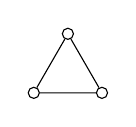
\begin{tikzpicture}[scale=0.5,every node/.style={node,inner sep=0.5mm},yshift=-2cm]
                \node (1) at (90:1) {};
                \node (2) at (-30:1) {};
                \node (3) at (-150:1) {};
                \draw (1) -- (2) -- (3) -- (1);
            \end{tikzpicture}
        }{\binom{n}{3} (p^3 - p^6)}
        + \underset{
            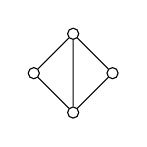
\begin{tikzpicture}[scale=0.5,every node/.style={node,inner sep=0.5mm},yshift=-1.7cm]
                \node (1) at (90:1) {};
                \node (2) at (-90:1) {};
                \node (3) at (-180:1) {};
                \node (4) at (0:1) {};
                \draw (1) -- (2) -- (3) -- (1) -- (4) -- (2);
            \end{tikzpicture}
        }
        {\binom{n}{3} \cdot 3 \cdot (n-3) (p^5 - p^6)}
        \leq n^3 p^3 + n^4 p^5.
    \end{equation*}

    Suppose first $p = \mathcal{o}(\frac{1}{n})$, i.e.\ $np \to 0$. Then by Markov,
    \begin{equation*}
        \mathbb{P}(X = 0) = 1 - \mathbb{P}(X \geq 1) \geq 1 - \mu \to 1 \text{ as } n \to \infty.
    \end{equation*}

    Suppose instead $p = \omega(\frac{1}{n})$ so $n p \to \infty$. Then with Chebyshev,
    \begin{equation*}
        \frac{\sigma^2}{\mu^2} \leq \frac{1}{\mu^2} (n^3 p^3 + n^4 p^5) \sim \frac{36}{n^6 p^6} (n^3 p^3 + n^4 p^5) = \frac{36}{(np)^3} + \frac{36}{n\cdot np} \to 0 \text{ as } n \to \infty. \qedhere
    \end{equation*}
\end{proof}




\begin{nthm}\label{thm:41}
    There exists a function $d: \mathbb{N} \to \mathbb{N}$ such that a.e.\ $G \in \mathcal{G}(n,p)$ has $\omega(G) \in \{d-1,d,d+1\}$ (where $d = d(n)$).
\end{nthm}
\begin{proof}[Proof sketch]
    \textbf{(Currently missing).}
\end{proof}

\begin{ncor}\label{cor:42}
    Almost every $G \in \mathcal{G}(n,p)$ has
    \begin{equation*}
        \chi(G) \geq (1 + o(1))\frac{n \log \frac{1}{q}}{2 \log n}
    \end{equation*}
    where $q = 1-p.$
\end{ncor}
\begin{proof}
    Let $G \in \mathcal{G}(n,p)$. Then $\overline{G} \in \mathcal{G}(n,q)$.
    So by \Cref{thm:41}, with probability tending to 1 as $n \to \infty$ we have
    \begin{align*}
        \omega(\overline{G}) &\sim \frac{2 \log n}{\log \frac{1}{q}} \\
        \implies \alpha(G) &\sim \frac{2 \log n}{\log \frac{1}{q}}\\
        \implies \chi(G) &\geq \frac{|G|}{\alpha(G)} \sim \frac{n \log \frac{1}{q}}{2 \log n}. \qedhere
    \end{align*}
\end{proof}



\clearpage
\section{Algebraic Methods}



























\subsection{The Chromatic Polynomial}










\begin{nthm}[Cut-fuse relation]\label{thm:43}
    Let $G$ be a graph, $e \in E(G)$, $k \geq 1$. Then $f_G(k) = f_{G-e}(k) - f_{G/e} (k)$.
\end{nthm}
\begin{proof}
    Let $e = uv$. Let $c$ be a $k$-colouring of $G-e$.
    If $c(u) \neq c(v)$ then $c$ is a $k$-colouring of $G$ and every $k$-colouring of $G$ arises uniquely like this.
    If $c(u) = c(v)$ then $c$ yields a $k$-colouring of $G/e$ and every $k$-colouring of $G/e$ arises uniquely like this.
    \begin{equation*}
        f_{G-e}(k) = f_G(k) + f_{G/e} (k). \qedhere
    \end{equation*}
\end{proof}
\begin{ncor}\label{cor:44}
    Let $G$ be a graph. Then $f_G$ is a polynomial.
\end{ncor}
\begin{proof}
    Induction on $e(G)$. For $e(G) = 0$, $f_G(k) = k^{|G|}$.
    For $e(G) > 0$, pick $e \in E(G)$. Then $f_{G-e}$, $f_{G/e}$ are polynomials by the induction hypothesis and hence $f_G = f_{G-e} - f_{G/e}$ is a polynomial.
\end{proof}













\begin{ncor}\label{cor:45}
    If $|G| = n$, $e(G) = m$ then
    \begin{equation*}
        f_G(X) = X^n - m X^{n-1} + \dotsc
    \end{equation*}
\end{ncor}
\begin{proof}
    Induction on $e(G)$. If $e(G)=0$, then $f(X) = X^n$, as required.
    For $e(G) > 0$, pick $e \in E(G)$.
    Then
    \begin{align*}
        f_G(X) &= f_{G-e}(X) - f_{G/e}(X) = (X^r (m-1) X^{n-1} + \dotsc) - (X^{n-1} + \dotsc) \\
               &= X^n - m X^{n-1} + \dotsc \qedhere
    \end{align*}
\end{proof}
\subsection{Eigenvalues}































\begin{nthm}\label{thm:46}
    Let $G$ be a graph, $\Delta(G) = \Delta$, $\lambda$ an eigenvalue of $G$.
    Then $|\lambda| \leq \Delta$.
    Moreover if $G$ is connected then $\Delta$ is an eigenvalue $\iff G$ is $\Delta$-regular; in this case $\Delta$ has multiplicity 1 and eigenvector $\left(\begin{smallmatrix}1\\1\\  \vphantom{\int\limits^x}\smash{\vdots}\\1\end{smallmatrix}\right)$.
\end{nthm}
\begin{proof}
    Let $A$ be the adjacency matrix and $x$ an eigenvector with eigenvalue $\lambda$.
    Let $i$ be such that $|x_i|$ is maximal. Without loss of generality, $x_i = 1$ and $\forall j, |x_j| \leq 1$.
    Then
    \begin{align*}
        |\lambda| &= |\lambda x_i| = |(A x)_i| = \left|\sum_{j=1}^n A_{ij} x_j\right| = \left|\sum_{j \in \Gamma(i)} x_j\right| \\
                  &\leq \sum_{j \in \Gamma(i)} |x_j| \leq d(i) \leq \Delta.
    \end{align*}

    Assume now $G$ is connected.
    ($\Leftarrow$). If $G$ is $\Delta$-regular then clearly $(1,\dotsc,1)^T$ is an eigenvector with eigenvalue $\Delta$.

    ($\Rightarrow$). Suppose $\Delta$ is an eigenvalue. Then taking $\lambda = \Delta$ in previous:
    \begin{equation*}
        \Delta = (Ax)_i = \sum_{j \in \Gamma(i)} x_j.
    \end{equation*}
    Hence $d(i) = \Delta$ and $\forall j \in \Gamma(i), x_j=1$.
    Repeat: $\forall j \in \Gamma(i)$ we have $d(j) = \Delta$ and $\forall k \in \Gamma(j)$, $x_k = 1$.
    Continuing, as $G$ connected, $\forall k, d(k) = \Delta$ and $x_k = 1$.
\end{proof}
\subsection{Strongly Regular Graphs}












\begin{nthm}[Rationality condition]\label{thm:47}
    Let $G$ be $(k,a,b)$-strongly regular.
    Then
    \begin{equation*}
        \frac{1}{2} \left\{ (n-1) \pm \frac{(a-b)(n-1) + 2k}{\sqrt{(b-a)^2 - 4(b-k)}}\right\} \in \mathbb{Z}.
    \end{equation*}
\end{nthm}
\begin{proof}
    Let $A$ be the adjacency matrix of $G$.
    Let $|G|=n$.
    By \Cref{thm:46}, $k$ is an eigenvalue of multiplicity 1 with eigenvector $(1,1,\dotsc,1)^T = v$.

    What about other eigenvalues?
    Let $\lambda \neq k$ be an eigenvalue with eigenvector $x$. Now
    \begin{equation*}
        (A^2)_{ij} =
        \begin{cases}
            k & \text{if } i = j \\
            a & \text{if } i \sim j \\
            b & \text{if } i \nsim j
        \end{cases}
    \end{equation*}
    Thus $A^2 = k I + aA + b(J-I-A)$ where $J$ is the matrix with a $1$ in every place.
    Applying this to $x$, and noting that $x \perp v$, giving $J x = 0$, we get $\lambda^2 x = k x + a \lambda x - b x - b \lambda x$.
    Also $x \neq 0$, so $\lambda^2 + (b-a) \lambda + (b-k) = 0$.

    So the remaining eigenvalues are
    \begin{equation*}
        \lambda = \frac{(a-b) + \sqrt{(b-a)^2 - 4(b-k)}}{2} \text{ and } \mu = \frac{(a-b) - \sqrt{(b-a)^2 - 4(b-k)}}{2}
    \end{equation*}
    with multiplicities $r,s$ say, respectively.

    Now $A$ is diagonalizable so
    \begin{align}
        r + s + 1 &= n \label{eq:24.1} \\
        \shortintertext{and $\Tr A = 0$ so}
        \lambda r + \mu s + k &= 0 \label{eq:24.2}
    \end{align}
    Now take $\lambda \times \eqref{eq:24.1} - \eqref{eq:24.2}$: $(\lambda - \mu) s = \lambda(n-1) + k$.

    We have $\lambda-\mu = \sqrt{(b-a)^2 - 4(b-k)}$ so
    \begin{align*}
        s &= \frac{1}{2} \left\{ (n-1) + \frac{(a-b)(n-1) + 2k}{\sqrt{(b-a)^2 - 4(b-k)}}\right\} \\
        \shortintertext{and so}
        r &= \frac{1}{2} \left\{ (n-1) - \frac{(a-b)(n-1) + 2k}{\sqrt{(b-a)^2 - 4(b-k)}}\right\}. \qedhere
    \end{align*}
\end{proof}

\end{document}